\chapter{Конструкторская часть}

В данном разделе будет представлена схема алгоритма кластеризации методом k-средних и также будет рассмотрен способ распараллеливания алгоритма. Кроме того будет проанализирована вычислительная сложность алгоритма.

\section{Разработка алгоритмов}

На рисунке \ref{img:standard} приведена схема алгоритма кластеризации методом k-средних. 


\begin{figure}[H]
	\begin{center}
		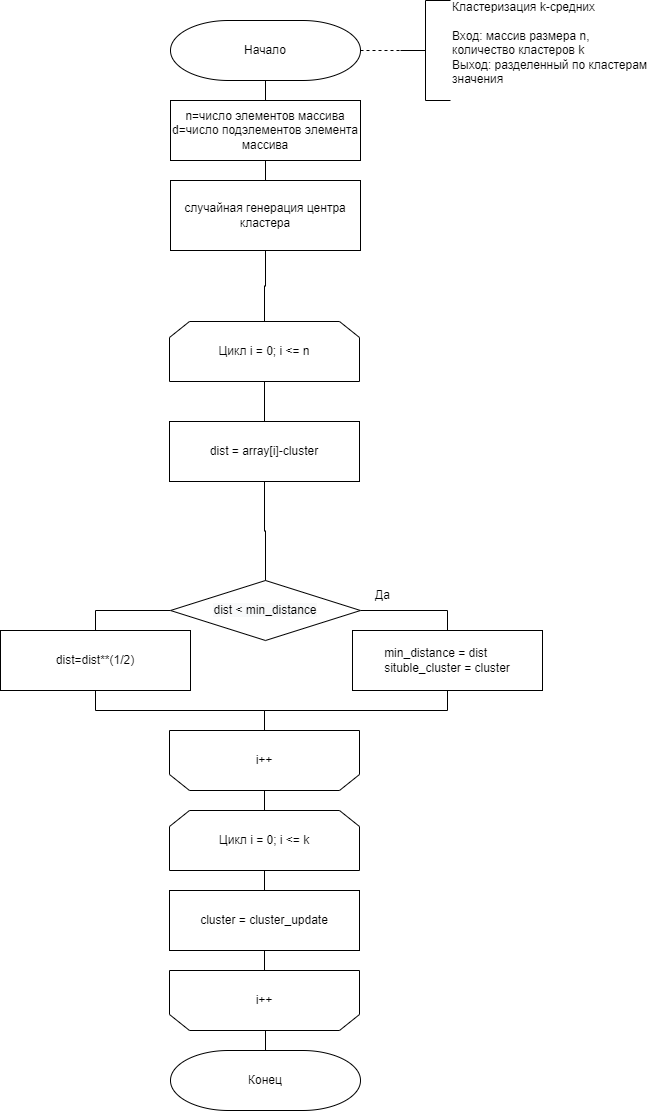
\includegraphics[scale=0.6]{img/standart.png}
	\end{center}
	\captionsetup{justification=centering}
	\caption{Алгоритм кластеризации методом k-средних}
	\label{img:standard}
\end{figure}


\section{Распараллеливание программы}

Распараллеливание программы должно ускорять время работы. 
Это достигается за счет реализации параллельных потоков в узких участках программы.
В алгоритме кластеризации методом k-средних данным участком будет являться участок, в котором происходит подсчет расстояния от элемента массива до центра кластера.



\section{Вычислительная сложность}

Алгоритм k-средних линейно зависит от всех своих факторов: от количества документов, количества кластеров, количества
терминов и количества итераций. 
Для сохранения линейной сложности  $(O(|D|))$  при  комбинировании с иерархическим с целью эффективного задания начальных
центроидов кластеров, предлагается квадратичный иерархический алгоритм
применить к выборке документов размером $\sqrt{|D|}$






\section{Вывод}

Была представлена схема алгоритма кластеризации. Был рассмотрен способ рспараллеливания алгоритма. Также была проанализированна вычислительная сложность.
